\chapter{Conclusions and Future Work}
\label{chap:conclusion}
In this chapter, we conclude our work. We begin by answering our research questions, then summarize our findings and outline future work.

\textbf{TODO}: go over research questions.

\subsection{Performance Improvements}
\label{performance-improvements}
Throughout the research for this thesis, we identified several promising ideas for future investigation. The following sections dive into some of these ideas.

\subsubsection{Enabling GRO within XDP}
\label{subsubsec:enabling-gro-within-xdp}
The performance benefits of GRO, stemming from reduced per-packet overhead within the Linux network stack, can be similarly extended to XDP. Figure~\ref{fig:gro-offload-with-xdp} demonstrates that the \texttt{XDP\_SKB} hook's invocation after \ac{GRO} processing makes it a suitable point to reuse existing \ac{GRO} logic. This stands in contrast with \texttt{XDP\_DRV}, which would necessitate moving the \ac{GRO} logic directly into the driver. With respect to enabling this change, according to Bianconi et al.~\cite{xdp_multibuff_2019}, initial work towards this integration is already in progress. A key enabler for this progress is the increasing support for XDP Fragments~\cite{af_xdp_driver_support} across various drivers.

\begin{figure}
	\centering
	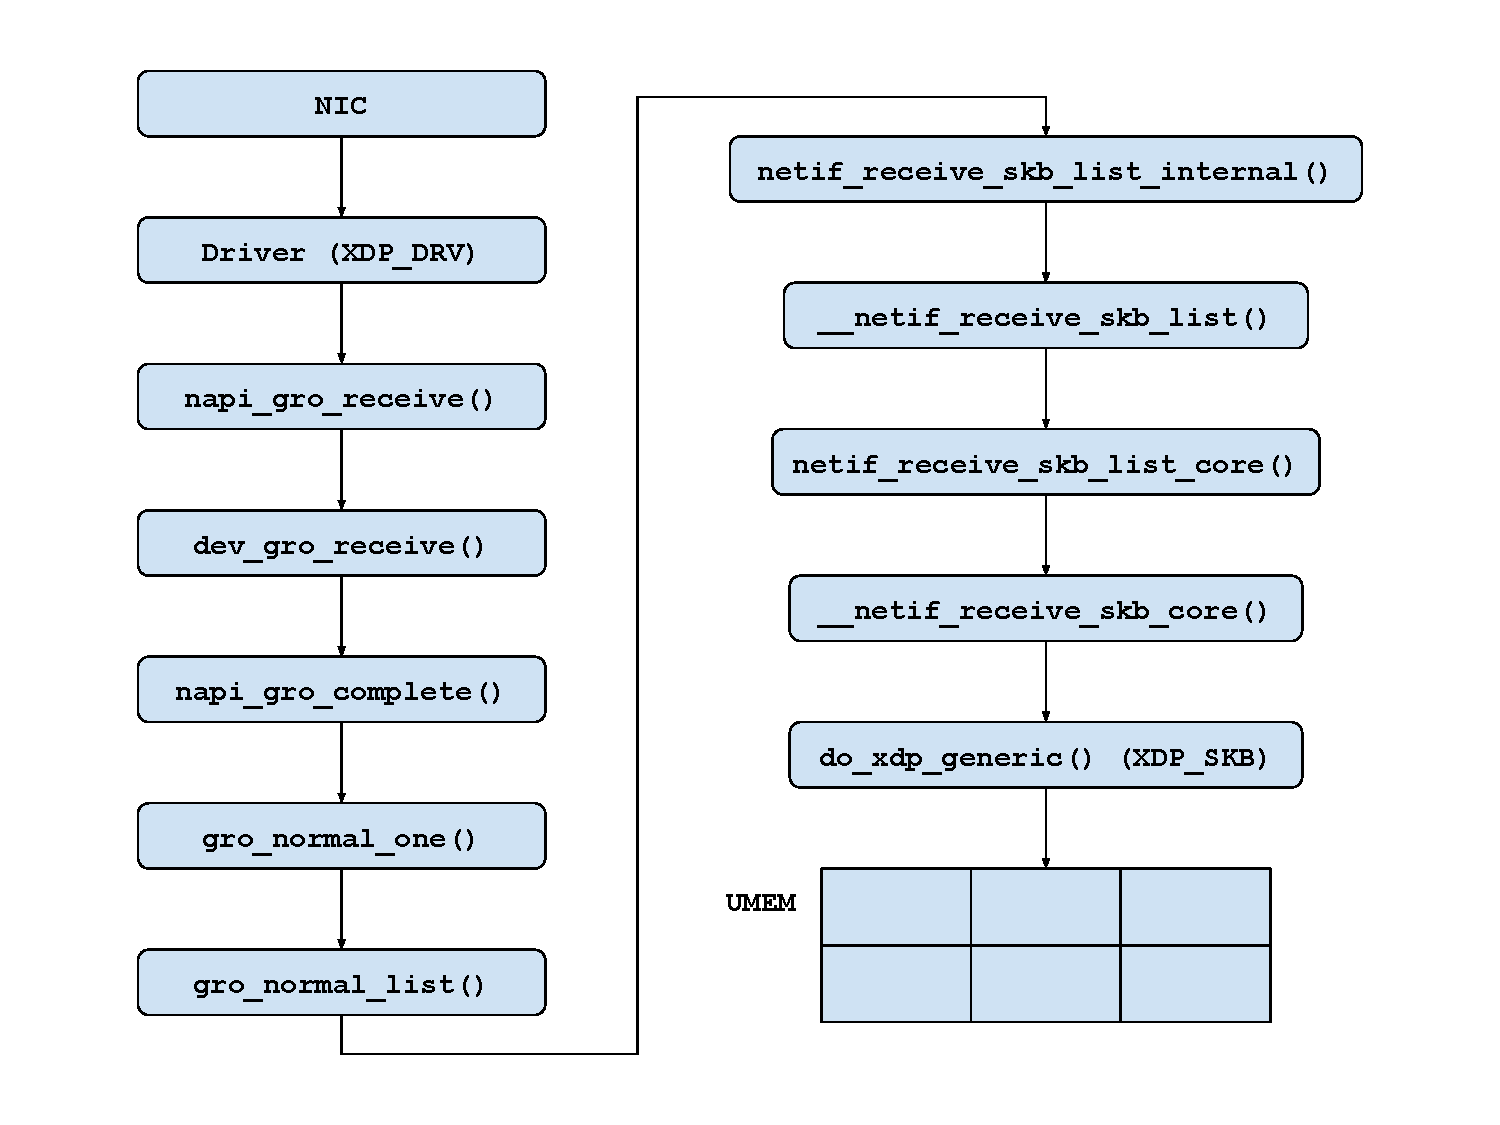
\includegraphics[width=.85\linewidth]{pics/gro-with-xdp.pdf}
	\caption[\ac{GRO} Offload with XDP.]{GRO Offload with XDP.}
	\label{fig:gro-offload-with-xdp}
\end{figure}

\subsubsection{Increasing the TX Batch Size}
\label{subsubsec:increasing-tx-batch-size}
One potential modification to MsQuic for enhanced transmit (TX) performance involves increasing the TX ring's batch size. In the MsQuic version 2.4.7 used for our measurements, the \texttt{CxPlatDpRawTxEnqueue} function currently reserves only a single descriptor from the TX queue when sending data~\footnote{\href{https://github.com/microsoft/msquic/blob/a6fe43d7928dc550b2f24599a2769df0358f963d/src/platform/datapath_raw_xdp_linux.c\#L1141}{datapath\_raw\_xdp\_linux.c, line 1141}}. As demonstrated by Karlsson et al.~\cite{2018AFXDPPerf}, larger TX batch and ring sizes significantly boost throughput in simple 64-byte packet benchmarks. While this doesn't directly translate to QUIC's MTU-sized packets, it indicates a promising direction. Implementing this change would require substantial refactoring to the MsQuic \ac{XDP} datapath logic.

\subsubsection{Encryption \ac{NIC} Hardware Offload}
\label{subsubsec:encryption-hw-offload}
Finally, as highlighted by Jaeger et al.~\cite{quic_on_the_highway}, encryption and decryption are the second largest consumers of CPU resources after packet I/O. Consequently, enabling hardware offload for these tasks would significantly impact performance. MsQuic is currently focused on enabling such offload capabilities~\footnote{https://github.com/microsoft/msquic/issues/4780}, with a proposal already describing the necessary steps for hardware vendors~\footnote{https://github.com/microsoft/net-offloads/blob/main/quic-encryption-offload.md}. Exploring this area could thus be a valid approach to improving throughput.